\chapter{Organization and Planning}

\section{Internal Structure}
In order to build a work strategy, the project is divided in tasks that will be described later on. As the different tasks are strongly interrelated, the project members have decided to follow a hierarchy. Every task is developed by a small team composed of two to five people depending on the amount of work that the task requires and its complexity.

Each small team has to have a coordinator which has two principal functions. The first one is to manage the group so he / she is responsible for the good organization and progression of the task. The second is that he / she is the voice of the team. That means that the coordinator is the one who represents his / her work team when transferring information to the other group coordinators and the project managers and vice versa.

Over all the teams Boyan Naydenov is the project manager who ensures the project progress and manages people for major decisions. Finally, Silvia Gonz\'{a}lez is the secretary in charge to write and delivery the minutes and agendas of each meeting. She is also in charge of the organization and storage of all the documents in BSCW.

The final organization of the team has been:
 
\begin{figure}[H]
\centering
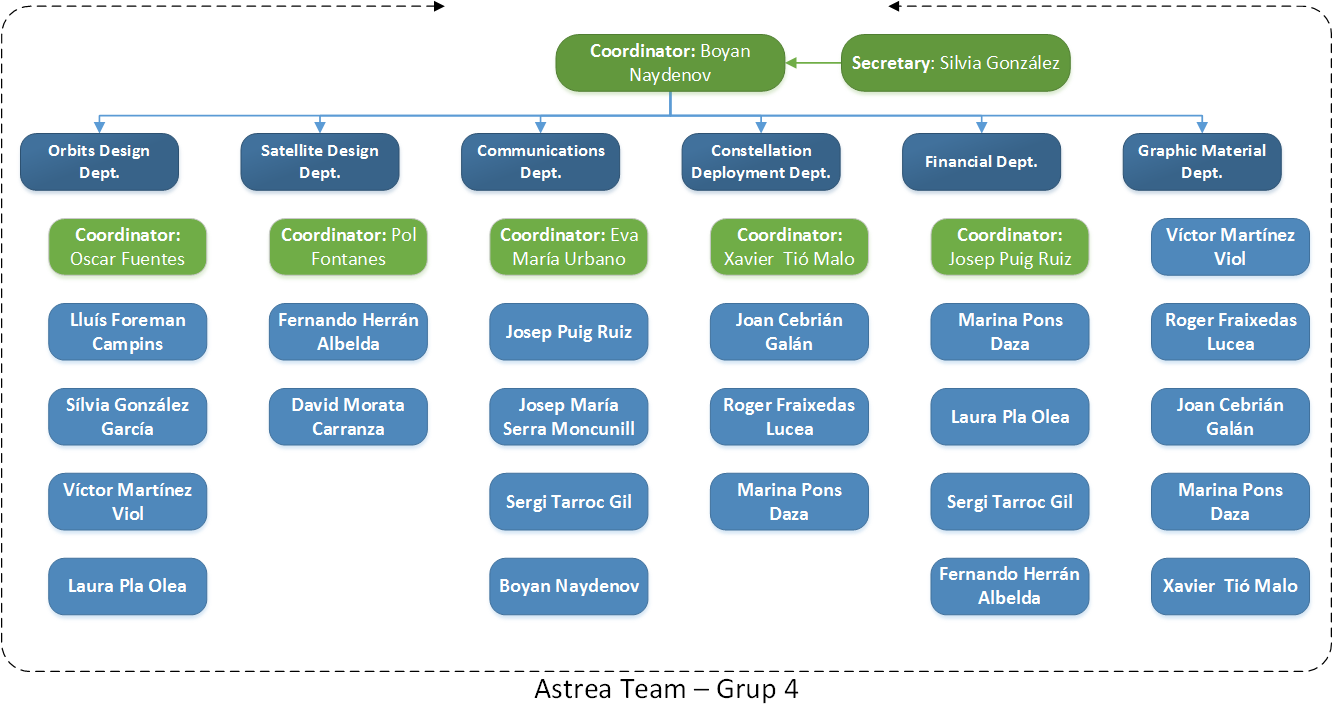
\includegraphics[width=15cm,height=15cm,keepaspectratio]{organigram-team.png}
\caption{Roles and Responsibilities}
\end{figure}

\section{Documents organisation}
The Astrea team has \textbf{17 members} so it is essential to define a protocol to organize all the documents and information found to take advantage of resources. 

The main internal communication tool used is \textit{Slack} which is a platform specialized in team communication. \textit{Slack} defines itself as a real-time messaging, archiving and searching tool for modern teams which is interesting for us since it allows the group to communicate at all times for punctual doubts and small decisions. For major decisions a meeting date will be specified using doodle. Communication between the customer and project manager will be carried out via e-mail. Weekly meetings with the customer are scheduled every Thursday and will be formalized through the agenda.

Moreover, to share documents two platforms are used: \textit{Slack} and \textit{BSCW}. Slack is used just for some discussion while \textit{BSCW} is the main information storage because information and documents are stocked and organized in folders. Hence, it is really helpful for keeping track of the proper progress of the work.

Besides, the text editor used to develop the project is the \textit{Latex} text processor which combined with \textit{Git} allows the team to work remotely on a same document without overriding other's work.  Git is just on of the many available \textit{Version Control System} out there. It keeps track of the changes done to the documents, so it is very easy to go back in case something goes wrong. Also, it avoids overwriting other's work. This features seem to be essential if a smooth workflow is to be assured in such a big team.

Finally, Git is combined with Slack and with Latex. The work-flow achieved doing this is the following:

\begin{itemize}
\item Someone is about to write some conclusions in the report. He/she checks if their local folder (repository) is synced  with the online repository. That is done through a simple terminal command. If there is new text, it will be added to their local folder.
\item The user works on the document with \textit{Latex} and applies some changes.
\item The user finishes and wants to upload the new changes to the online repository so he/she just writes a command on the terminal and then, his or her local repository is synced with the on-line one. In the case that someone has done some changes before the user finishes, then  \textit{Git} will inform the user that he or she has to take actions in order to merge the files safely.
\item Once the updates have been applied to the on-line repository, \textit{Slack} notifies automatically all the team that the current user has made some changes.
\item Finally, the user also publish the document on BSCW so that files arrive to the costumer as well.
\end{itemize}

\begin{figure}[H]
\minipage{0.5\textwidth}
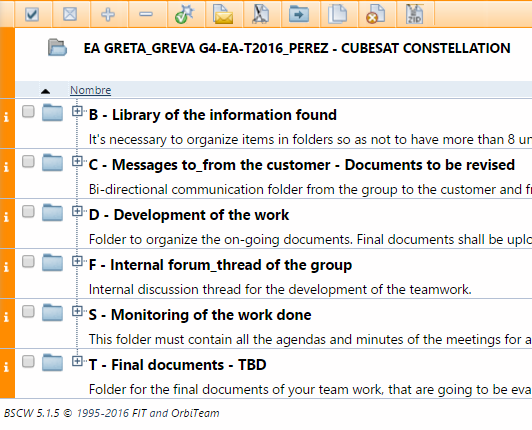
\includegraphics[width=\linewidth]{bscw.png}
\caption{BSCW}\label{fig:bscw}
\endminipage\hfill
\minipage{0.5\textwidth}
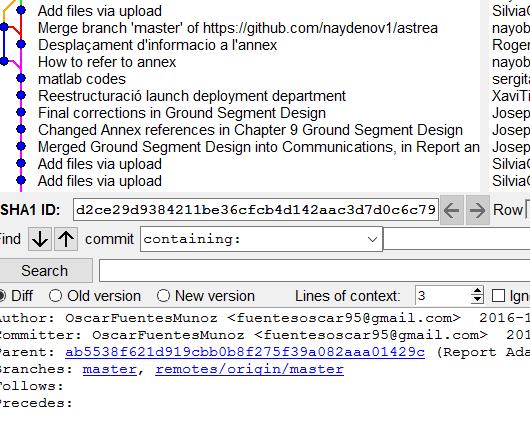
\includegraphics[width=\linewidth]{git.png}
\caption{Git commits, viewed with Gitk}\label{fig:git}
\endminipage
\end{figure}

\begin{figure}[H]
\minipage{0.5\textwidth}%
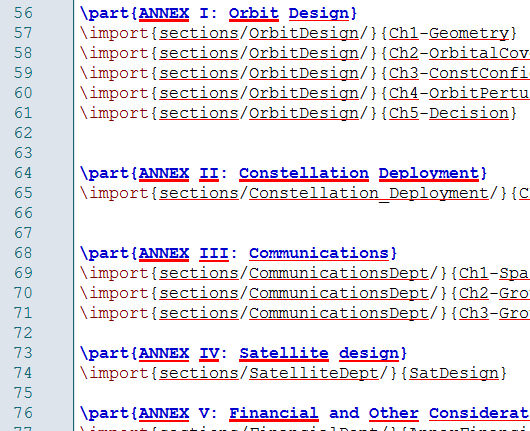
\includegraphics[width=\linewidth]{latex.png}
\caption{Texmaker, Latex.}\label{fig:latex}
\endminipage
\minipage{0.5\textwidth}%
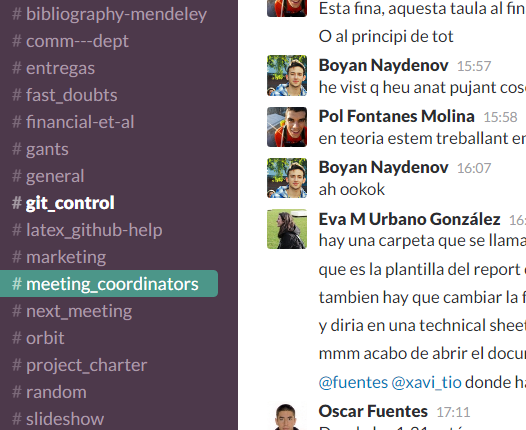
\includegraphics[width=\linewidth]{slack.png}
\caption{Slack}\label{fig:slack}
\endminipage
\end{figure}

The applied system has helped in achieving high modularity and has saved the team many hours of unimportant work.

\section{Planning}

\subsection{Tasks identification from work breakdown structure (WBS)}
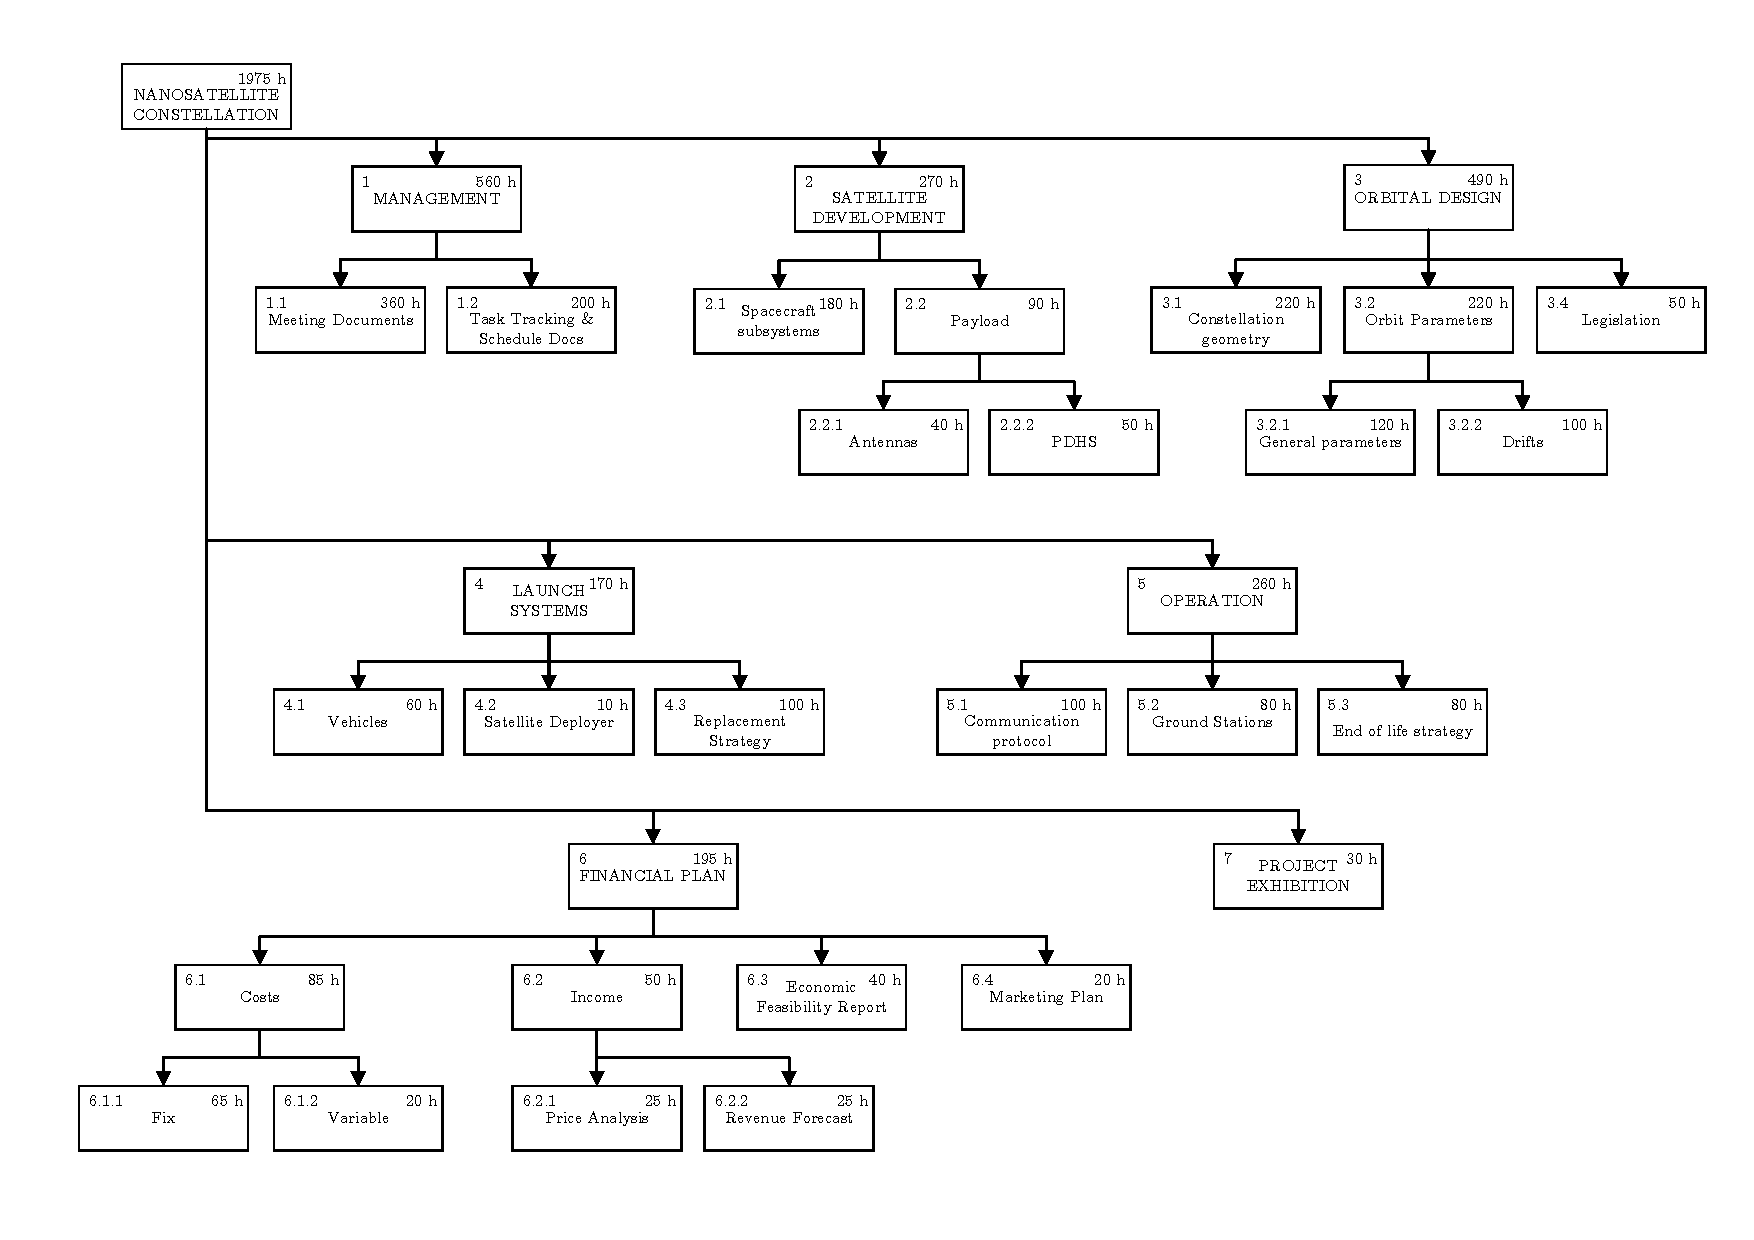
\includepdf[pages={1-}, landscape=true]{./external_pdf/G4-PC-WBS-10-04.pdf}
%\begin{figure}[h]
%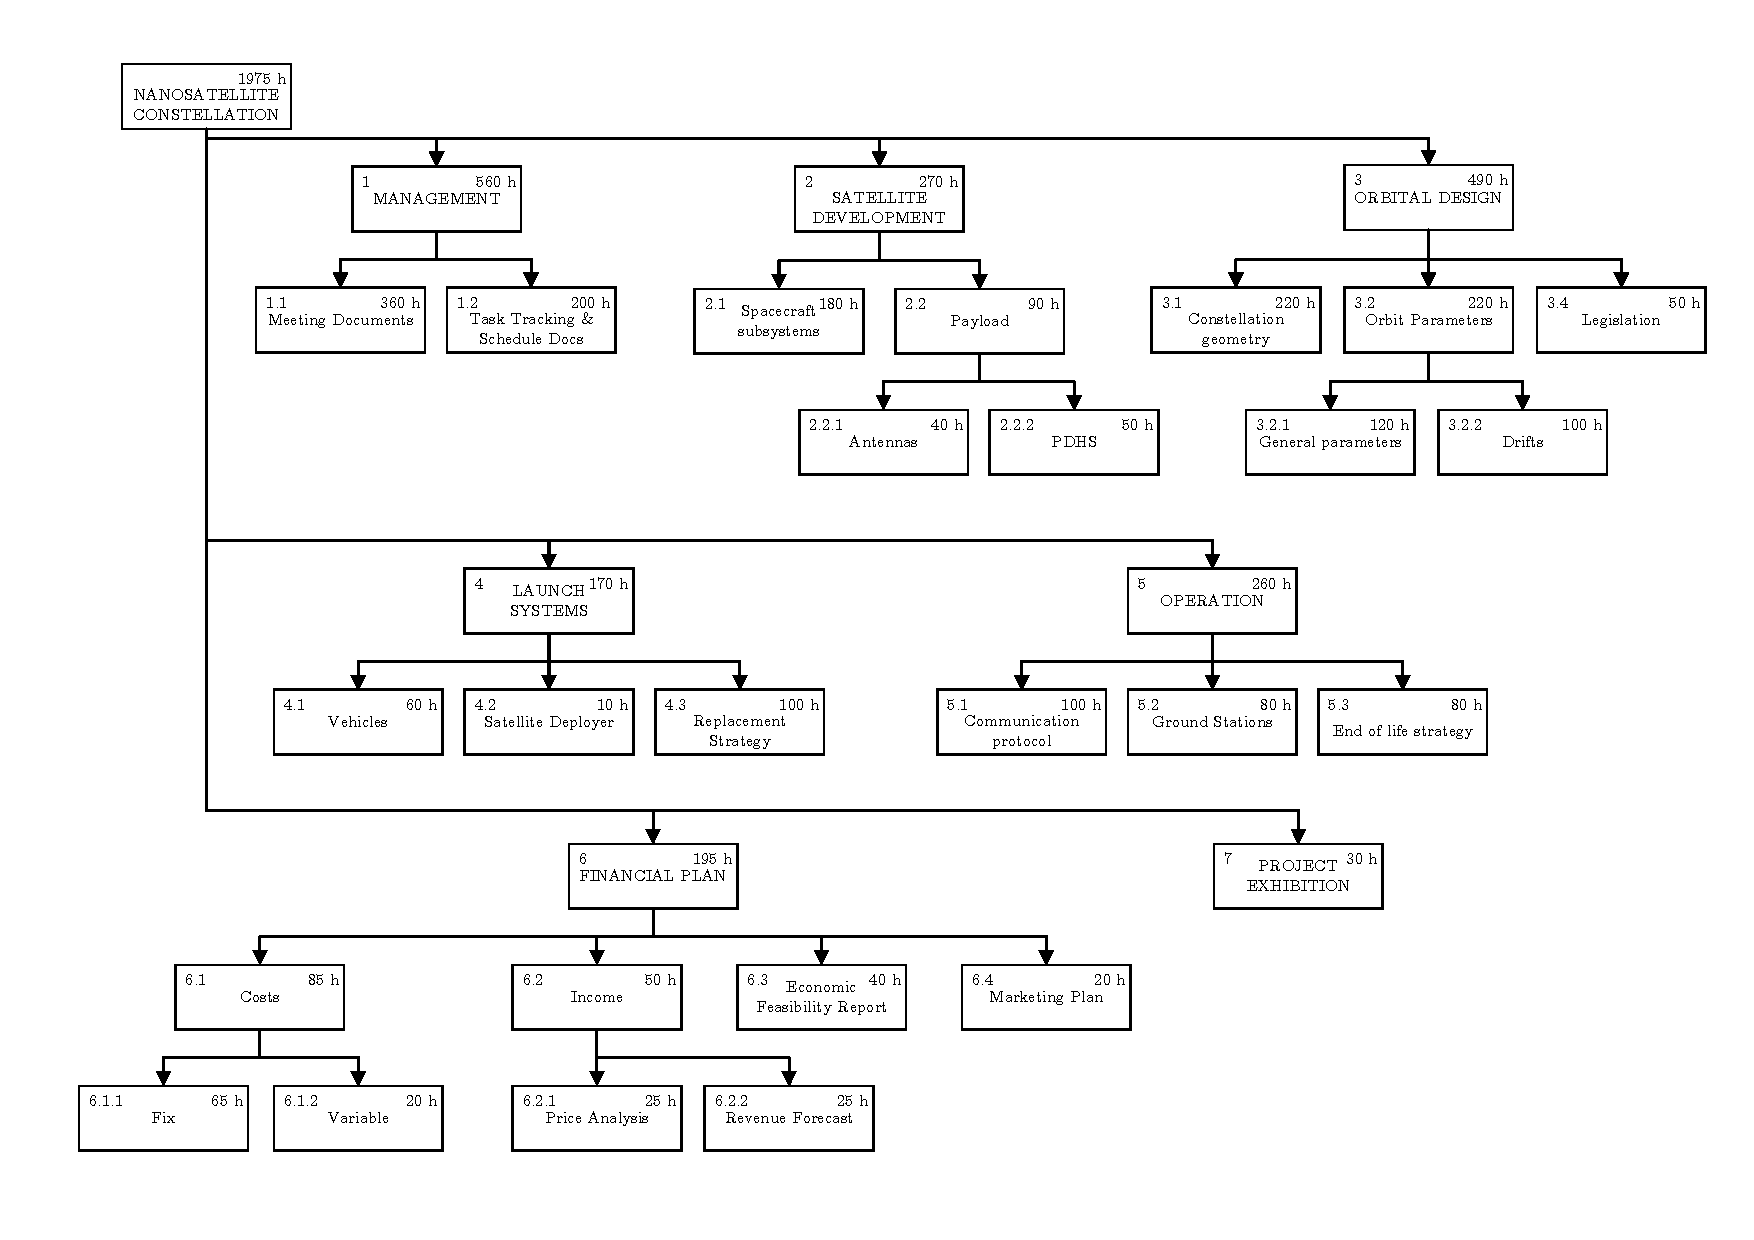
\includegraphics[width=1.1\textwidth]{./external_pdf/G4-PC-WBS-10-04.pdf}
%\end{figure}

\pagebreak

\subsection{Interdepency relationships, human resources and level of effort}
\begin{longtable}{ | p{1.3cm} | p{5cm} | p{3cm} | p{3.5cm} |}
\hline

\textbf{ID }& \textbf{Work Package} & \textbf{Time (h)} & \textbf{Prelations} \\ \hline
\multicolumn{4}{|c|}{\textbf{1.Management}} \\ \hline
1.1 & Meetings Documents & 360 &   \\ \hline
1.2 & Tasks tracking and scheduling & 200 & BB - 1.1 \\ \hline
\multicolumn{4}{|c|}{\textbf{2.Satellite}} \\ \hline
2.1 & Spacecraft Subsystems & 180 & BB - 1 \\ \hline
2.2.1 & Payload antenna & 40 & BB - 2.1 \\ \hline
2.2.2 & PDHS & 50 & BB - 2.1 \\ \hline
\multicolumn{4}{|c|}{\textbf{3. Orbital Design}} \\ \hline
3.1 & Constellation geometry & 220 & BB - 1 \\ \hline
3.2.1 & General parameters & 120 & BF - 3.1 \\ \hline
3.2.2 & Drifts & 100 & BB - 3.2.1 \\ \hline
3.3 & Legislation & 50 & BB - 1, 2, 3.1\\ \hline
\multicolumn{4}{|c|}{\textbf{4. Launch Systems}} \\ \hline
4.1 & Vehicle & 60 & BF - 4.3 \\ \hline
4.2 & Satellite Deployer & 10 & BF - 4.3  \\ \hline
4.3 & Replacement Strategy & 100 & BB - 1  \\ \hline
\multicolumn{4}{|c|}{\textbf{5. Operations}} \\ \hline
5.1 & Communication protocol & 100 & BB - 1 \\ \hline
5.2 & Ground station & 80 & BF - 5.1 \\ \hline
5.3 & End of life Strategy & 80 & BF - 5.2 \\
\hline
\multicolumn{4}{|c|}{\textbf{6. Financial Plan}} \\ \hline
6.1.1.1 & Maintenance Cost Analysis & 10 & BF - 3,4,5; BB - 2 \\ \hline
6.1.1.2 & Insurance Cost Analysis & 15 & BF - 3,4,5; BB - 2  \\ \hline
6.1.1.3 & Administration Cost Analysis & 15 & BF - 3,4,5; BB - 2 \\ \hline
6.1.1.4 & Taxes Cost Analysis  & 25 & BF - 3,4,5; BB - 2 \\ \hline
6.1.2.1 & Manufacturing Cost Report & 10 & BF - 3,4,5; BB - 2 \\ \hline
6.1.2.2 & Launching Cost Report  & 10 & BF - 3,4,5; BB - 2 \\ \hline
6.2.1 & Price Analysis & 25 & BF - 3,4,5; BB - 2 \\ \hline
6.2.2 & Revenue Forecast & 25 & BF - 3,4,5; BB - 2 \\ \hline
6.3 & Economic Feasibility Report & 40 & BF - 3,4,5; BB - 2  \\ \hline
6.4 & Marketing Plan & 20 & BF - 6.2.1,6.2.2 \\ \hline
\multicolumn{4}{|c|}{\textbf{7. Project Exhibition}} \\ \hline
7 & Project Exhibition &30 & BF - 3 \\ \hline
\caption{Prelations and Time} \\
\end{longtable}

\section{Scheduling}
Along the past four months, the costumer has been periodically informed, on a weekly basis, about the project situation regarding the scheduling. This has been done using \textit{Microsoft Project} with which a \textit{Gantt} was done. This Gantt has been updated by the team coordinators in a modular way since every department managed their own Gantt, while the project manager kept track of all of them together.Samples of this documents can be found at the \textit{Scheduling Deliverable}. There, it can be seen in red the critical path, among many other indicators. Furthermore, Microsoft Project was also used for generating weekly reports, showing a very short and clear summary regarding the overall situation. It showed the late tasks, the percentage of completion of the departments and the finished tasks during the last few days.